% ----------------------------------------------------------
\chapter{Resultados}
% ----------------------------------------------------------
Neste capitulo falaremos das nossas implementações e de nossos resultados com algumas delas. As estruturas\footnote{Afim de a aplicação ser agnóstica de sistema, utilizamos o programa pipenv que permite criar ambientes Python com as dependencias necessárias. Instruções de uso estão disponíveis no arquivo README do projeto. \url{https://github.com/lrdass/theia}} foram implementadas na linguagem Python, e para validação visual preferimos imagens SVG por serem fáceis de interpretar e de gerar imagens teste. Além da implementação das estruturas desenvolvemos dois casos de testes para validar as estruturas. O primeiro é uma aplicação onde há um mapa com movimento livre com inúmeros pontos. A ideia deste programa era validar tanto a aplicação para jogos 2D quanto 3D. Para um jogo 2D, poderíamos substituir cada ponto por texturas do jogo, e teríamos um mapa virtualmente infinito em dimensões. E portanto, buscamos neste capitulo validar que podemos consultar no plano grandes ordens de grandeza de pontos sem grandes impactos na performance. Validamos esta ideia mostrando os tempos de consulta para grandes valores de pontos. O segundo programa é um mapa do Brasil com grande resolução de segmentos e movimento de câmera livre por este mapa. Validamos a aplicação mostrando que seria inviável ter uma aplicação de tempo real sem as estruturas utilizadas. Construímos cada uma das estruturas de dados apresentadas no texto e cada uma delas tem métodos auxiliares para construir figura SVG com pontos aleatórios com janelas aleatórias, e a construção da árvore em cima do arranjo de pontos desta imagem e a saída do programa como outra figura SVG com os pontos dentro da janela indicados com a cor verde.Todas as estruturas foram construídas visando apenas a consulta em janela. Portanto como demonstrado no texto nos atentamos apenas aos métodos de construção e consulta. As estruturas de consulta para segmentos por sua vez foram construídas, como visto no trabalho até aqui, para consultas das bordas e portanto trabalham em conjunto com as estruturas de consultas de pontos. Para interpretarmos as imagens utilizamos a biblioteca \textit{xml}\footnote{Biblioteca built-in Python para lídar com arquivos XML \url{https://docs.python.org/3/library/xml.etree.elementtree.html}} e interpretamos as figuras SVG como XML.Usamos a mesma biblioteca tanto para a leitura quanto escrita das figuras após a consulta. Nos resultados obtidos utilizamos um computador com as configurações: Processador Intel® Core™ i7-7500U\footnote{Referencia completa do CPU utilizado \url{https://ark.intel.com/content/www/br/pt/ark/products/95451/intel-core-i7-7500u-processor-4m-cache-up-to-3-50-ghz.html}} com 8GB de RAM DDR4 2666MHz.

\section{Aplicação árvore de intervalos}\label{cap:application-points}
Em uma aplicação tridimensional poderíamos construir cenas arbitrariamente grandes de tal forma que organizaríamos os objetos da cena $3D$ com uma árvore de alcance de 3 dimensões. Consultaríamos nesta árvore, portanto, o cubo representado pela câmera como na Figura \ref{fig:3d-query-example}. Reportando somente quais estruturas estão dentro da janela e então enviaríamos para o pipeline gráfico \ref{cap:cg} para desenharmos na tela. Podemos pensar em uma limitação para um jogo que precisa manter todos os objetos geométricos no pipeline. O número de objetos geométricos seria limitado pela memória do pipeline. 
A partir destas constatações podemos recriar este comportamento construindo uma árvore de alcance tridimensional com todos os seus objetos, e carregamos para memória da placa de video apenas o que é retornado da consulta. Necessitando de apenas uma tela de carregamento para construir a árvore.

\begin{figure}[h!]
    \centering
    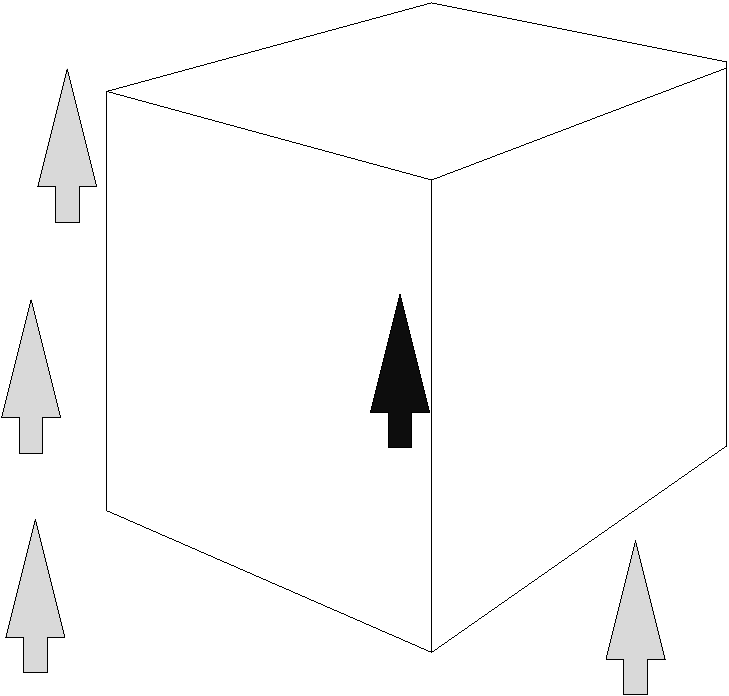
\includegraphics[scale=0.4]{images/3d-query-example.pdf}
    \caption{Exemplo de cena tridimensional com uma consulta retornando apenas os objetos dentro da janela. Considere as setas como figuras tridimensionais no espaço. E o cubo como a janela de consulta.}
    \label{fig:3d-query-example}
\end{figure}

Para justificarmos esta aplicação, construímos uma versão simplificada do problema em duas dimensões visto na Figura \ref{fig:application_example_dots}. Criamos aleatoriamente pontos no plano e construímos uma árvore de alcance bidimensional. Em cada laço de execução do programa, consultamos a árvore com a janela, e desenhamos apenas os pontos dentro da janela. A solução trivial deste problema sem as árvores de alcance é consultar cada ponto e então desenha-lo e deixar o algoritmo de recorte \cite{folley01} desenhar na tela. Porem, ainda iteraria sobre estes para poder constatar que não estão na janela. Enquanto utilizando a árvore, temos uma maneira eficiente de consultar e desenhar apenas os pontos dentro da janela.

\begin{figure}[h!]
\centering
\begin{minipage}{.5\textwidth}
  \centering
  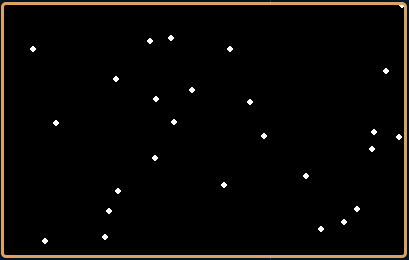
\includegraphics[width=.8\linewidth]{images/Captura de tela de 2021-04-16 11-43-23.png}
 
  \label{fig:sub1}
\end{minipage}%
\begin{minipage}{.5\textwidth}
  \centering
  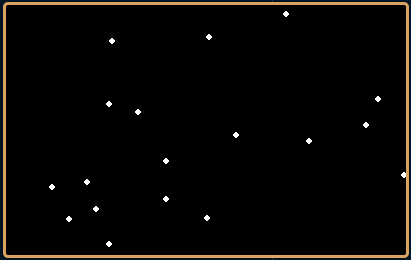
\includegraphics[width=.8\linewidth]{images/Captura de tela de 2021-04-16 11-43-35.png}
  
  \label{fig:sub2}
\end{minipage}
\caption{Aplicação construída com pontos no plano e consultas em tempo real}
\label{fig:application_example_dots}
\end{figure}

Como jogos são aplicações de tempo real, temos que pensar em restrições de tempo. Jogos modernos tem objetivos de entregar entre 30 e 60 quadros por segundo. Considerando o pior caso temos $\frac{1}{30} \approx 0.0334$ segundos para computações entre cada quadro.

\begin{table}[h!]
\centering
\begin{tabular}{|c c c |} 

 \hline
 Pontos & Média do Tempo (s) & Desvio Padrão (s) \\%$\sigma$ \\
 \hline
 1000  & $0.00012955069541931$  & $1.3212002262037\times 10^{-5}$ \\
\hline
 10000  & $0.00013832251230876$  & $2.0937153306017\times 10^{-5}$ \\
\hline
 100000  & $0.00015597189626386$  & $2.8073955196226\times 10^{-5}$ \\
\hline
\end{tabular}
\caption{Tabela comparativa do número de pontos e o tempo para reportar os pontos em uma janela proporcional ao tamanho do conjunto de pontos testado}
\label{table:1}
\end{table}

\begin{table}[h!]
\centering
\begin{tabular}{|c c |} 

 \hline
 Incremento médio tempo consulta(s) para cada $10^{n} $ pontos & Desvio Padrão (s) \\%$\sigma$ \\
 \hline
 $0,00001321$  & $ 6.276986896593 \times 10^{-6}$ \\
\hline
\end{tabular}
\caption{Há um incremento médio de 13,21 microssegundos para cada $10^{n}$ pontos na consulta }
\label{table:2}
\end{table}

Com base na Tabela \ref{table:1} temos bastante confiança de que a estrutura de dados está dentro do tempo limite de computação para cada quadro desenhado, até mesmo aumentando o número de pontos. Mostrando que o crescimento com um fator de $10^n$ o tempo da consulta ainda permanece na casa dos $0.1$ milissegundos.

\section{Aplicação árvore de segmentos}\label{cap:application-segment}
Em aplicações de tempo real pode ser que exista apenas um objeto com grande complexidade. Programas que permitem ilustração em tempo real, por exemplo, estão mais interessados em conhecer se determinado segmento do objeto sendo desenhado está dentro da janela. Ou mapeamento tridimensional de um sistema cardiovascular em tempo real em que temos uma malha de um único objeto com grande complexidade e, para visualizá-lo, temos que carregar apenas um recorte deste objeto complexo. Em OpenGL \cite{opengl} temos um arranjo com as posições dos vértices chamado $Vertex Array$ e um segundo arranjo que contém uma ordem de cada vértice para formar os triângulos chamado $Element Array$. Podemos portanto interpretar estes dois arranjos e construir os segmentos pois sabemos que cada aresta de um triângulo é um segmento. E assim utilizar estes para construir e consultar com a árvore de segmentos. Para simplificarmos este problema tridimensional, desenvolvemos uma aplicação mostrado na Figura \ref{fig:execut1} (à direita) que navega pelo mapa do Brasil com alta resolução de segmentos em tempo real. 

\begin{table}[h!]
\centering
\parbox{.5\linewidth}{
\centering
\begin{tabular}{| c c |} 
 \hline
 Média do Tempo (s) & Desvio Padrão (s) \\%$\sigma$ \\
 \hline
 $0.005857$  & $0.003753$ \\
\hline
\end{tabular}
\caption{Utilizando a estrutura de dados para consultar os segmentos}
\label{table:3}
}
\parbox{.5\linewidth}{
\centering
\begin{tabular}{| c c |} 
 \hline
 Media do Tempo (s) & Desvio Padrão (s) \\%$\sigma$ \\
 \hline
 $0.148667$  & $0.017494$ \\
\hline
\end{tabular}
\caption{Sem a estrutura de dados consultando linearmente}
\label{table:4}
}
\end{table}

A consulta linear está inviável para uma aplicação de tempo real demonstrado na Tabela \ref{table:4}. Imaginando a mesma restrição de 30 quadros por segundo tendo $\frac{1}{30} \approx 0.0334$ segundos para calcular um quadro seria inviável atingir o objetivo sem a árvore de segmentos. A consulta linear alcançaria no máximo $\frac{1}{0.1487} \approx 6.72$ quadros por segundo nos nossos experimentos.
